%% LaTeX-Beamer template for KIT design
%% by Erik Burger, Christian Hammer
%% title picture by Klaus Krogmann
%%
%% version 2.1
%%
%% mostly compatible to KIT corporate design v2.0
%% http://intranet.kit.edu/gestaltungsrichtlinien.php
%%
%% Problems, bugs and comments to
%% burger@kit.edu

\documentclass[18pt]{beamer}


%% SLIDE FORMAT

% use 'beamerthemekit' for standard 4:3 ratio
% for widescreen slides (16:9), use 'beamerthemekitwide'
\usepackage{listings}
\usepackage{templates/beamerthemekit}
% \usepackage{templates/beamerthemekitwide}
\usepackage{color}
\definecolor{editorGray}{rgb}{0.95, 0.95, 0.95}
\definecolor{editorOcher}{rgb}{1, 0.5, 0} % #FF7F00 -> rgb(239, 169, 0)
\definecolor{editorGreen}{rgb}{0, 0.5, 0} % #007C00 -> rgb(0, 124, 0)
\usepackage{upquote}
\lstdefinelanguage{JavaScript}{
	morekeywords={typeof, new, true, false, catch, function, return, null, catch, switch, var, if, in, while, do, else, case, break},
	morecomment=[s]{/*}{*/},
	morecomment=[l]//,
	morestring=[b]",
	morestring=[b]'
}

\lstdefinelanguage{HTML5}{
	language=html,
	sensitive=true, 
	alsoletter={<>=-},
	otherkeywords={
		% HTML tags
		<html>, <head>, <title>, </title>, <meta, />, </head>, <body>,
		<canvas, \/canvas>, <script>, </script>, </body>, </html>, <!, html>, <style>, </style>, ><
	},  
	ndkeywords={
		% General
		=,
		% HTML attributes
		charset=, id=, width=, height=,
		% CSS properties
		border:, transform:, -moz-transform:, transition-duration:, transition-property:, transition-timing-function:
	},  
	morecomment=[s]{<!--}{-->},
	tag=[s]
}

\lstset{%
	% Basic design
	backgroundcolor=\color{editorGray},
	basicstyle={\small\ttfamily},   
	frame=l,
	% Line numbers
	xleftmargin={0.75cm},
	numbers=left,
	stepnumber=1,
	firstnumber=1,
	numberfirstline=true,
	% Code design   
	keywordstyle=\color{blue}\bfseries,
	commentstyle=\color{darkgray}\ttfamily,
	ndkeywordstyle=\color{editorGreen}\bfseries,
	stringstyle=\color{editorOcher},
	% Code
	language=HTML5,
	alsolanguage=JavaScript,
	alsodigit={.:;},
	tabsize=2,
	showtabs=false,
	showspaces=false,
	showstringspaces=false,
	extendedchars=true,
	breaklines=true,        
	% Support for German umlauts
	literate=%
	{Ö}{{\"O}}1
	{Ä}{{\"A}}1
	{Ü}{{\"U}}1
	{ß}{{\ss}}1
	{ü}{{\"u}}1
	{ä}{{\"a}}1
	{ö}{{\"o}}1
}
%% TITLE PICTURE

% if a custom picture is to be used on the title page, copy it into the 'logos'
% directory, in the line below, replace 'mypicture' with the 
% filename (without extension) and uncomment the following line
% (picture proportions: 63 : 20 for standard, 169 : 40 for wide
% *.eps format if you use latex+dvips+ps2pdf, 
% *.jpg/*.png/*.pdf if you use pdflatex)

\titleimage{learn-coding-online}

%% TITLE LOGO

% for a custom o on the front page, copy your file into the 'logos'
% directory, insert the filename in the line below and uncomment it

%\titlelogo{mylogo}

% (*.eps format if you use latex+dvips+ps2pdf,
% *.jpg/*.png/*.pdf if you use pdflatex)

%% TikZ INTEGRATION

% use these packages for PCM symbols and UML classes
% \usepackage{templates/tikzkit}
% \usepackage{templates/tikzuml}

% the presentation starts here

\title[Javascript Basics]{Spielentwicklung}
\subtitle{Wie man ein einfaches Spiel mit HTML5 und Javascript entwickelt}
\author{Lena, Kristin, Charlotte}

% Bibliography

\usepackage[citestyle=authoryear,bibstyle=numeric,hyperref,backend=biber]{biblatex}
\addbibresource{templates/example.bib}
\bibhang1em

\begin{document}

% change the following line to "ngerman" for German style date and logos
\selectlanguage{ngerman}

%title page
\begin{frame}
\titlepage
\end{frame}

\section{Canvas Basics}

\begin{frame}[fragile]{Was ist HTML5 Canvas}
\begin{itemize}
	\item HTML5 Element um Grafiken auf eine Webseite zu zeichnen
	\item Wird in HTML mit \textless canvas\textgreater  -Tag eingefügt 
	\item Ist nur ein Container 
	\item Zeichnen erfolgt aus Javascript-code
\end{itemize}
\end{frame}

\begin{frame}[fragile]{Canvas HTML Element einfügen}
\begin{lstlisting}
<div>
<canvas id="game" width="600" height="300"></canvas>
</div>
\end{lstlisting}
\begin{lstlisting}
<script>paintGame();</script>
\end{lstlisting}
\end{frame}

\begin{frame}{Das Koordinatensystem in Canvas}
\begin{figure}[htb]
	\centering
	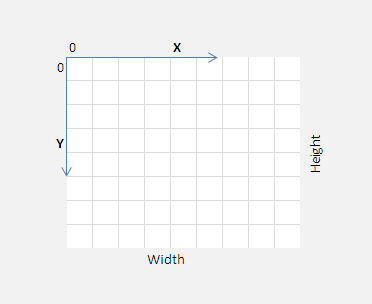
\includegraphics{logos/canvascos}
\end{figure}
\end{frame}

\begin{frame}[fragile]{Wie zeichnet man Vierecke}
\begin{lstlisting}
//um in JS auf das Canvas zuzugreifen
canvas = document.getElementById("game");
context = canvas.getContext("2d");

//gefülltes Viereck
context.fillStyle = color;
context.fillRect(x,y,breite,hoehe);

//ungefülltes mit Rand
context.strokeStyle = color;
context.strokeRect(x, y, breite, höhe);
\end{lstlisting}

\end{frame}

\begin{frame}{Jetzt ihr!}
\begin{itemize}
	\item F"ugt ein Canvas Element zum HTML-Dokument hinzu
	\item Ruft die Funktion Paint game am Ende des Bodys aus dem HTML auf
	\item Implementiert die Funktion paintGame() 
	\item Fügt verschiedene Vierecke dem Canvas Element hinzu
\end{itemize}
\end{frame}

\begin{frame}[fragile]{Javascript Objekte}
\begin{itemize}
	\item Komponenten, wie Vierecke bestehen eigentlich aus mehreren zusammenhängenden Informationen (Koordinaten, Breite, Höhe...)
	\item Also alle Informationen in einem Objekt speichern 
	\item Objekt für gefüllte Viereck und für Text ist jeweils bereits in Javascript Datei vorhanden 
	
\end{itemize}
 \begin{lstlisting}
var component = new component(20, 20, "red", 50, 50);
//width, height, color, x, y
component.update();
var textComponent = textComponent("30px", "Consolas", "black", 280, 40, "Hallo");
//testSize, font, color, x, y, text
textComponent.update();
\end{lstlisting}
\end{frame}


\begin{frame}[fragile]{Javascript Objekte - Jetzt ihr!}
\begin{itemize}
	\item Ersetzt eure zuvor gezeichneten Vierecke durch Objekte
	\item Fügt Text hinzu
	\item speichert alle Objekte in einer globalen Liste
	

\end{itemize}
\begin{lstlisting}
var component = new component(20, 20, "red", 50, 50);
//width, height, color, x, y
component.update();
var textComponent = textComponent("30px", "Consolas", "black", 280, 40, "Hallo");
//testSize, font, color, x, y, text
textComponent.update();
\end{lstlisting}
\end{frame}



\section{Spielbasics}

\begin{frame}{Die Idee - Was wir hier Programmieren wollen}
\begin{figure}[htb]
	\centering
	
\includegraphics[width=1\textwidth]{logos/game}
\end{figure}
\end{frame}

\begin{frame}{Was ist eine Gameloop?}
\begin{itemize}
	\item Um das Feld zu aktualsieren wird das Spielfeld nach wenigen Millisekunden neugezeichnet
	\item Mit startIntervall kann eine Methode in einem bestimmten Zyklus immer wieder aufgerufen werden 
	\item Zum beenden stopIntervall() aufrufen
	\item Im Zyklus wird immer die Funktion updateGameArea() aufgerufen\\ \( \Rightarrow \) alles was gezeichnet werden muss, soll da rein
\end{itemize}
\end{frame}

\begin{frame}{start, stop, neustart, clear}
\begin{itemize}
	\item Start besteht aus 2 Schritten: Werte zurück setzen und Inverall starten
	\item Stop muss nur stopInverall ausführen
	\item Neustart besteht auch aus 2 Schritten: stop und start
	\item Clear: leert das Canvas und wird zum Starten aufgerufen, aber auch bei jedem neuzeichnen des Spielfelds

\end{itemize}
\end{frame}

\begin{frame}{start, stop, neustart, clear}
\begin{itemize}
	\item Wieso habt ihr zuvor die Objekte in einer Liste gespeichert?
	\item Wie kann man den Spielablauf mit einer gameloop als Ablauf zeichnen?
	
\end{itemize}
\end{frame}


\section{Der Spieler}
\begin{frame}{Spieler einfügen}
\begin{itemize}
	\item Spieler ist rotes Viereck mit Höhe und Breite 20px und Startpunkt bei x=y=50px
	\item Wird als Objekt global gespeichert (redGamePiece)
	\item Wird beim Start angelegt und in der Loop-Funktion dann geupdatet
\end{itemize}
\end{frame}

\section{Der Spieler}
\begin{frame}{Spieler bewegen}
\begin{itemize}
	\item Durch Aufruf der Funktion initKeyHandling() kann der Spieler hoch und runter bewegt werden und eine Schussfunktion aufgerufen werden
\end{itemize}
\end{frame}


\begin{frame}{initKeyHandling() - BONUS}
\begin{itemize}
	\item Es wird auf zwei Events vom Browser reagiert: Taste runterdr"ucken und Taste loslassen
	\item Das Event speichert als keyCode die Nummer der betroffenen Taste
	\item Relevant für uns: 38 (up), 40 (down) und 32(Leertaste)
	
\end{itemize}
\end{frame}

\begin{frame}{initKeyHandling() - BONUS}
\begin{itemize}
	\item Bewegung wird gestartet in dem die Componente des Spielers eine speedY gesetzt bekommt (hier +/-3)
	\item Bewegung wird beendet in dem die Geschwindigkeit wieder auf 0 gesetzt wird
	\item Beim nächsten Update der Komponente wird diese um speedY bewegt und neugezeichnet
	\item Wird die Leertaste runtergedr"uckt wird die function shoot() aufgerufen
\end{itemize}
\end{frame}

\begin{frame}{Schießen implementieren}
\begin{itemize}
	\item Eine Komponente wird erzeugt. Wo? 
	\item Diese wird mit den anderen Geschossen in der Liste runningGamePieces gespeichert
	\item Das Geschoss benötigt eine Geschwindigkeit in X-Richtung (positiv oder negativ?) (hier 5)
	\item In der Loopfunktion müssen diese so lang sie sichtbar sind immer geupdatet werden
	\item Wie?
\end{itemize}
\end{frame}

\begin{frame}[fragile]{Schießen implementieren}
\begin{itemize}
	\item In der Funktion updateGameArea() (also der Loopfunktion)
	\item Liste der Geschosse durchgehen in einer Liste (runningGamePieces)
	\item Wenn piece.x über den Rand überspringen
	\item Ansonsten: update() aufrufen und in einer Liste der noch gültigen Geschosse speichern
	\item Am Ende Liste der runningGamePieces ersetzen
\end{itemize}
\end{frame}

\begin{frame}[fragile]{Schießen implementieren}
\begin{lstlisting}
for(var i = 0; i<runningGamePieces.length; i++) {
	var piece = runningGamePieces[i];
	if(!piece) {
		continue;
	}
	if(piece.x > canvasXSize) {
	continue;
	}
	piece.update();
	newRunningGamePieces.push(piece);
}
runningGamePieces = newRunningGamePieces;
\end{lstlisting}
\end{frame}


\section{Die Gegner}
\begin{frame}{Zufällige Gegner}

Gegner sollen randomisiert erscheinen.
Parameter die Randomisiert sein soll:
\begin{itemize}
	\item Gr"o"se
	\item Geschwindigkeit
	\item H"ohe
\end{itemize}
\end{frame}

\begin{frame}{Randomisieren}
\begin{itemize}
	\item Math enthält vordefinierte mathematischen Funktionen wie Math.abs(), Math.floor(), Math.sin()
	\item Mit Math.random() bekommt man eine zuf"allige Kommazahl zwischen 0 und 1 (0 inklusive, 1 nicht)
	\item Wie kann man mit Math.random() eine zuf"allige Zahl zwischen einem Minimum und einem Maximum machen?
	
\end{itemize}
\end{frame}

\begin{frame}[fragile]{Randomisieren}
\begin{lstlisting}
function random(min, max) {
	return Math.random()*(max-min+1)+min;
}
\end{lstlisting}
\end{frame}

\begin{frame}[fragile]{Gegner erzeugen - BONUS}
\begin{itemize}
	\item 1. Zuf"allige Geschwindigkeit generieren (zwischen 0.8 und 4)
	 \item 2. Zuf"allige Gr"o"se der Gegener erzeugen (z.B. zwischen 10 und 40 pixel)  
	\item 3. Zuf"alliegen Spawn Punkt, also die y-Koordinate, erzeugen (zwischen 0 und unterem Ende - Gegenergr"o"se) 
	\item 4. Gegner als neue Komponente erzeugen
	\item 5. Geschwindkeit in X Richtung setzen(als Negativen Wert)
	\item 6. Componente der Liste an Gegner hinzufügen	
\end{itemize}
\end{frame}

\begin{frame}{Gegner in der Loop hinzufügen}
\begin{itemize}
	\item Basis: Liste opponentGamePiece mit allen Komponenten
	\item Ziel: alle Gegner Bewegen und neuzeichnen 
	\item Wo \& Wann: in der Loop-Funktion, also in updateGameArea()
	\item Idee: Alle Gegner durchgehen mit einer Schleife und jeweils update() aufrufen
	\item Mehr zu beachten? 
\end{itemize}
\end{frame}

\begin{frame}{Gegner in der Loop hinzufügen}
\begin{itemize}
	\item Idee: Alle Gegner durchgehen mit einer Schleife und jeweils update() aufrufen
	\item Zu beachten:
	\item Linker Rand
	\item Kollisionen (was soll dann passieren?) 
\end{itemize}
\end{frame}

\begin{frame}[fragile]{Gegner in der Loop hinzufügen}
\begin{lstlisting}	
for(var i = 0; i<opponentGamePieces.length; i++) {
	var opponentPiece = opponentGamePieces[i];
	//überprüfe ob der Angreifer am linken Rand ist
	if(opponentPiece.x <= 0) {
		stopInterval();
		break;
	}
	//TODO: Kollosionen
	//Wenn nicht getroffen wurde: 
	opponentPiece.update();
	newOpponentGamePieces.push(opponentPiece);
}
opponentGamePieces = newOpponentGamePieces;
	
\end{lstlisting}
\end{frame}

\section{Kollisionen}
\begin{frame}{Kollisionen erkennen}
\begin{itemize}
	\item Implementiert als Funktion eines Objekt
	\item Aufruf über obj.carshWith(otherObj)
	\item Wie funktioniert das?
\end{itemize}

\end{frame}

\begin{frame}{Kollisionen verarbeiten}
Erweiterung des Codes, bei dem die Gegner in der Loop hinzugefügt werden.
Zwei verschiedene Kollisionen überprüfen:
\begin{itemize}
	\item Gegner mit Spieler
	\item Geschoss mit Gegner
\end{itemize}
\end{frame}

\begin{frame}[fragile]{Gegner mit Spieler}
In der Schleife die die Gegner aktualisiert
\begin{lstlisting}
	if(opponentPiece.crashWith(redGamePiece)) {
		stopInterval();
		break;
	}
\end{lstlisting}
\end{frame}

\begin{frame}{Geschoss mit Gegner}
In der Schleife die die Gegner aktualisiert
\begin{itemize}
	\item Idee: bestimme in der Schleife ob der Gegner mit einem Geschoss kollidiert ist
	\item Dazu: Pro Gegner werden jeweils alle Geschosse durchgegangen
	\item Bei Crash, speichern, Geschoss entfernen, score erhöhen, Gegner tauchen schneller auf und fortsetzen
	\item Bei Crash den Gegner nicht in die neue Gegnerliste hinzuf"ugen
\end{itemize}
\end{frame}

\begin{frame}[fragile]{Geschoss mit Gegner}
In der Schleife die die Gegner aktualisiert
\begin{lstlisting}
var crashed = false;
for(var j = 0; j<runningGamePieces.length; j++) {
	var piece = runningGamePieces[j];
	if(piece && opponentPiece.crashWith(piece)) {
		runningGamePieces[j] = null;
		crashed = true;
		score += 10;
		minOpponentFrequency -=2;
		continue;
	}
}
//nur wenn nicht gecrashed wird der Gegner wieder in die Liste aufgenommen
\end{lstlisting}
\end{frame}

\end{document}
